\documentclass{beamer}

\usepackage{xcolor}
\usepackage{amsmath,amssymb}
\usepackage{tikz}
\usepackage{tikz-cd}
\usepackage{graphicx}

\usetikzlibrary{shapes.geometric}

\tikzset{pics/.cd,
opencube/.style args={#1/#2/#3}{code={
\coordinate (O) at (0,0,0);
\coordinate (A) at (0,#2,0);
\coordinate (B) at (0,#2,#3);
\coordinate (C) at (0,0,#3);
\coordinate (D) at (#1,0,0);
\coordinate (E) at (#1,#2,0);
\coordinate (F) at (#1,#2,#3);
\coordinate (G) at (#1,0,#3);
%% Background
\draw[black,dotted] (O) -- (A);
\draw[black,dotted] (O) -- (C);
\draw[black,dotted] (O) -- (D);
% Forground
\draw[black,dashed] (A) -- (E) -- (F) -- (B) -- cycle;
\draw[black,dashed] (E) -- (D) -- (G) -- (C) -- (B);
\draw[black,dashed] (F) -- (G);

%\draw[black,dashed, blue] (O) -- (A) -- (E) -- (D) -- cycle;
%\draw[black,dashed] (O) -- (A) -- (B) -- (C) -- cycle;
%\draw[black,dashed] (D) -- (E) -- (F) -- (G) -- cycle;
%\draw[black,dashed] (C) -- (B) -- (F) -- (G) -- cycle;
%\draw[black,dashed] (A) -- (B) -- (F) -- (E) -- cycle;

}}}

\tikzset{pics/.cd,
linecube/.style args={#1/#2/#3/#4}{code={
\coordinate (OO) at (0,0,0);
\coordinate (AA) at (0,#2,0);
\coordinate (BB) at (0,#2,#3);
\coordinate (CC) at (0,0,#3);
\coordinate (DD) at (#1,0,0);
\coordinate (EE) at (#1,#2,0);
\coordinate (FF) at (#1,#2,#3);

\coordinate (GG) at (#1,0,#3);
%% Background
\draw[black,dashed] (OO) -- (AA);
\draw[black,dashed] (OO) -- (CC);
\draw[black,dashed] (OO) -- (DD);

\node at (0.5*#1,0.5*#2,0.5*#3) {#4};

% Foreground
\draw[black] (AA) -- (EE) -- (FF) -- (BB) -- cycle;
\draw[black] (EE) -- (DD) -- (GG) -- (CC) -- (BB);
\draw[black] (FF) -- (GG);

%\draw[black,dashed, blue] (O) -- (A) -- (E) -- (D) -- cycle;
%\draw[black,dashed] (O) -- (A) -- (B) -- (C) -- cycle;
%\draw[black,dashed] (D) -- (E) -- (F) -- (G) -- cycle;
%\draw[black,dashed] (C) -- (B) -- (F) -- (G) -- cycle;
%\draw[black,dashed] (A) -- (B) -- (F) -- (E) -- cycle;

}}}


\tikzset{pics/.cd,
shadedcube/.style args={#1/#2/#3/#4/#5}{code={
\coordinate (O) at (0,0,0);
\coordinate (A) at (0,#2,0);
\coordinate (B) at (0,#2,#3);
\coordinate (C) at (0,0,#3);
\coordinate (D) at (#1,0,0);
\coordinate (E) at (#1,#2,0);
\coordinate (F) at (#1,#2,#3);
\coordinate (G) at (#1,0,#3);
\draw[black,fill=#4!80] (O) -- (C) -- (G) -- (D) -- cycle;
\draw[black,fill=#4!30] (O) -- (A) -- (E) -- (D) -- cycle;
\draw[black,fill=#4!10] (O) -- (A) -- (B) -- (C) -- cycle;
\draw[black,fill=#4!20,opacity=0.8] (D) -- (E) -- (F) -- (G) -- cycle;
\draw[black,fill=#4!20,opacity=0.6] (C) -- (B) -- (F) -- (G) -- cycle;
\draw[black,fill=#4!20,opacity=0.8] (A) -- (B) -- (F) -- (E) -- cycle;
\node at (0.5*#1,0.5*#2,0.5*#3) {#5};
}}}
\tikzset{pics/.cd,
gridcube/.style args={#1/#2/#3/#4/#5/#6/#7}{code={
\coordinate (O) at (0,0,0);
\coordinate (A) at (0,#2,0);
\coordinate (B) at (0,#2,#3);
\coordinate (C) at (0,0,#3);
\coordinate (D) at (#1,0,0);
\coordinate (E) at (#1,#2,0);
\coordinate (F) at (#1,#2,#3);
\coordinate (G) at (#1,0,#3);

% Foreground
\draw[fill=#7!20] (A) -- (E) -- (F) -- (B) -- cycle;
\draw[fill=#7!40] (E) -- (F) -- (G) -- (D) -- cycle;
\draw[fill=#7!30] (B) -- (F) -- (G) -- (C) -- cycle;
%\draw[black] (E) -- (D) -- (G) -- (C) -- (B);
%\draw[black] (F) -- (G);

% lines
\foreach \ll in {1,...,#4} {
    \draw[black] (#1/#4*\ll,#2,0) -- (#1/#4*\ll,#2,#3) -- (#1/#4*\ll,0,#3);
}
\foreach \ll in {1,...,#5} {
    \draw[black] (0,#2/#5*\ll,#3) -- (#1, #2/#5*\ll,#3) -- (#1,#2/#5*\ll,0);
}
\foreach \ll in {1,...,#6} {
    \draw[black] (0,#2,#3/#6*\ll) -- (#1,#2,#3/#6*\ll) -- (#1,0,#3/#6*\ll);
}

}}}

%\pgfmathsetmacro{\xx}{0.5}

\mode<presentation>
% \setbeameroption{hide notes}
{
  %\usetheme{Madrid}
  \usetheme{metropolis}
% CSU COLORS
  \definecolor{csugreen}{HTML}{1C674F}
  \definecolor{csugold}{HTML}{B78E00}
    \definecolor{csured}{HTML}{E02F11}

  \definecolor{greenmain}{HTML}{00AF64}
  \definecolor{brick}{rgb}{.85,.1,.2}
  \colorlet{greenstruct}{greenmain!87.5!black}
  \usecolortheme[named=csugreen]{structure}
  % Change this in order to make the presentation look
  % different. Works just like a powerpoint template. 
  % Have your RA mess around until it looks nice.
  \setbeamercovered{dynamic}

  \useinnertheme{rectangles}
  
 %Other colors.

%   \definecolor{bluemain}{HTML}{0B61A4}
%   \definecolor{orangemain}{HTML}{AA6600}
%   \definecolor{redmain}{HTML}{E02F11}
%   \definecolor{redlight}{HTML}{FF9B73}
%   \definecolor{orangelight}{HTML}{FFC373}
%   \definecolor{cmugray}{RGB}{104,104,104}
%   \definecolor{cmulightgray}{RGB}{238,238,238}
%   \setbeamercolor{block body}{bg=cmulightgray}
%   \setbeamercolor{talktitle}{bg=csugreen,fg=white}
%   \setbeamercolor{block title alerted}{bg=csugold}
%   \setbeamercolor{block body alerted}{bg=orangelight}

}
\renewcommand{\footnoterule}{}
\renewcommand{\hat}[1]{\widehat{#1}}
\newcommand{\sourcenum}[3]{$^{\textcolor{bluemain} #1}$\let\thefootnote\relax
  \footnotetext{\begin{flush#2}\textcolor{bluemain}
      {\tiny $^{#1}$ #3}\end{flush#2}}} 
\newcommand{\source}[2]{\let\thefootnote\relax\footnotetext{\begin{flush#1}
      \textcolor{bluemain}{\tiny Source: #2}\end{flush#1}}}  


\DeclareMathOperator{\Span}{Span}
\DeclareMathOperator{\Pres}{Pres}
\DeclareMathOperator{\End}{End}
\newcommand{\bmto}{\rightarrowtail}

\usepackage{wasysym} 
\newcommand{\den}[1]{\Leftcircle\hspace*{-1mm}#1\hspace*{-1mm} \Rightcircle}

\begin{document}

\title{Tensor Clusters:\\The hard case}
\author{CC-BY 2021 James B. Wilson\\ Colorado State University}
%\date{\today}

\maketitle

%%%%%%%%%%%%%%%%%%%%%%%%%%%%%%%%%%%%%%%%%%%%%%%%%%%%%%%%
\section{Applications}

\subsection{Data science}
\begin{frame} 
    \begin{block}{Data}
        Results of measurement \& computation, e.g.\\[5pt]
        \centering
        \emph{Mercury is 2.5cm high in tube}.
    \end{block}

    \begin{block}{Information}
        data used to make a decision, e.g.\\[5pt]
        \centering
        \emph{Thermometer reads $38^{\circ}$F; I'll wear a coat.} 
    \end{block}
    

    \begin{block}{The Data Problem}
        Turn data into information.
    \end{block}

\end{frame}


\begin{frame}
    \frametitle{Nutrition Matrix}
    Nutrients$\times$Produce data collected and used on diet problems.
    \bigskip 

    \begin{tabular}{c|cccccc|}
             & Apple & Beef & Egg & Filbert & $\cdots$ & Strawberry \\
    \hline
    Carbs    & 13.8  & 1    & 2    & 4.8    & $\cdots$  & 7.7 \\
    Protein  & 0.3   & 20.7 & 17.1 & 3.9    &  & 0.7 \\
    Fat      & 0.2   & 7.4  & 14.4 & 1.3    &  & 0.3 \\
    $\vdots $ & $\vdots$ & & & & &\\
    \hline 
    \end{tabular} 

    \bigskip
    Substitute other examples\\
     minerals$\times$ mines, pollutants$\times$water-source, 
    keywords$\times$authors
\end{frame}

\begin{frame}[fragile]
    \frametitle{Nutrition Tensor}
    Reality is more complex...
    \begin{center}
        Nutrients $\times$ Produce $\times$ Farms $\times$ Water Source $\times$ Fertilizer
    \end{center}
    \centering
    \pgfmathsetmacro{\xx}{0.5}
    \begin{tikzpicture}[scale=1.5]
        \pic at (1.25,1.25,0) {
            linecube={3.75/2.5/1.75/{
                \begin{tikzpicture}
                    \foreach \x/\xc in {1/blue,2/red,3/green} {
                        \pic at (1.25*\x,1.25*1,0.25) {gridcube={1/0.75/1/4/3/4/{\xc}}};
                    }
                    \foreach \x/\xc in {1/purple,2/brown,3/teal} {
                        \pic at (1.25*\x,1.25*2,0.25) {gridcube={1/0.75/1/4/3/4/{\xc}}};
                    }
                \end{tikzpicture}
            }}        
        };
        \node[rotate=45] at (0.75,0.5,0) {Rain};
        \node[rotate=45] at (1.5,0.25,0) {Willamette};
        \node[rotate=45] at (2.5,0.25,0) {Deschutes};

        \node[rotate=-30] at (4.75,1,1) {{\small Crawford Farms}};
        \node[rotate=-30] at (4.75,0.9,0.5) {{\small Four Pines Ranch}};
        \node[rotate=-30] at (4.60,.9,0) {{\small Schlecter Farms}};
        \node[rotate=-30] at (4.75,0.8,-0.5) {{\small Thistledown Farms}};

        \node at (4,1.5,-1) {{\small Phosphate}};
        \node at (4,2,-1) {{\small Nitrogen}};
        
        \node (N) at (-1,2,-0.25) {{\small Nutrients}};
        \node (F) at (2,3,-0.75) {{\small Produce}};
        \draw[thick] (N) -- (1,1.25,0);
        \draw[thick] (N) -- (1,2.25,0);
        \draw[thick] (F) -- (1.5,2.5,-0.75);
        \draw[thick] (F) -- (2 ,2.5,-0.75);
        \draw[thick] (F) -- (2.5,2.5,-0.75);
    \end{tikzpicture}
    
\end{frame}

\begin{frame}

    \frametitle{First Approximation of Tensor}
        Fox coefficients $K$ and set $[n]=\{1,\ldots,n\}$.
\bigskip

        A \emph{hypermatrix} (some call it a ``tensor'') is a function
        $\Gamma:[d_1]\times \cdots\times [d_{\ell}]\to K$.

        \[K^{d_1\times\cdots\times d_{\ell}} = \{\Gamma:[d_1]\times \cdots\times [d_{\ell}]\to K\}.\]

    Technical matter: For general sets $X_1,\ldots, X_{\ell}$
    $\Gamma:X_1\times \cdots \times X_{\ell}\to K$ has \emph{finite support} (only finitely many nonzero values).
    
\end{frame}

\begin{frame} 
    Data collection chooses bases for convenience/practicality/instrumentation/safety/laws/...
    \begin{itemize}
        \item Measure each fruit, farm, fertilizer  separately
        \item Choose nutrients a lab can measure (Carbs, Sugar, Vit. A, Vit. B...)
    \end{itemize}

    \bigskip
    \textbf{Data collection is basis dependent;\\ 
    Likely some qualities of nutrition are basis independent.}

    \begin{block}{The Tensor-Data Problem}
        Find basis invariant properties of tensor data.\\
        (This is now a math problem!)
    \end{block}
    
\end{frame}


\begin{frame}

    \frametitle{Second Approximation of Tensor}

    A function $\langle \Gamma |:K^{X_1}\times \cdots \times K^{X_{\ell}}\bmto K$ where 
    \begin{align*}
        \langle \Gamma| u_1,\ldots, u_{\ell}\rangle 
        & = \sum_{x_1\in X_1} \cdots \sum_{x_{\ell}\in X_{\ell}} \Gamma_{x_1\cdots x_{\ell}} u_{1x_1}\cdots u_{\ell x_{\ell}}.
    \end{align*}

    {\color{magenta} $\bmto$?}  Just reminds me to tell you this is same ``multi-linear''
    \begin{align*}
        & (\forall a) & 
        \langle t|u_a+\lambda \tilde{u}_{a},u_{\bar{a}}\rangle 
        & = \langle t|u_a,u_{\bar{a}}\rangle 
        + \lambda \langle t|\tilde{u}_{a},u_{\bar{a}}\rangle 
    \end{align*}
    
\end{frame}



\begin{frame}
    \frametitle{Example: Find change of basis matrices to get clusters}
    \pgfmathsetmacro{\xx}{0.5}
	\begin{tikzpicture}
		
		\node (T) at (-4,0,0) {\begin{tikzpicture}
			\pic at (0,0,0) {shadedcube={2*\xx/2*\xx/2*\xx/gray/}};
			%\draw [->] (0,0,0) -- (5,0,0)
			\node[rotate=90] at (2*\xx,0.5*\xx,-1*\xx) {{\small users}};
			\node[rotate=45] at (-0.7*\xx,2*\xx,0) {{\small time}};
			\node at (0.2*\xx,-1*\xx,0*\xx) {{\small words}};
	
			\draw (0*\xx,2*\xx,0*\xx) rectangle (2*\xx,3.3*\xx,0*\xx);
	%        \draw (0*\xx,2*\xx,0*\xx) rectangle (2*\xx,4*\xx,0*\xx);
			\draw (0*\xx,0*\xx,2*\xx) --++ (0*\xx,2*\xx,0*\xx)
			   --++ (0*\xx,0*\xx,2*\xx) --++ (0*\xx,-2*\xx,0*\xx) -- cycle;
			\draw (2*\xx,0*\xx,0*\xx) --++ (2*\xx,0*\xx,0*\xx)
			   --++ (0*\xx,0*\xx,2*\xx) --++ (-2*\xx,0*\xx,0*\xx) -- cycle;
	
			\node[rotate=45,xslant=0.5] at (0*\xx,1*\xx,3*\xx) {{\small X}};
			\node at (1*\xx,2.7*\xx,0) {{\small Y}};
			\node[xslant=0.5] at (3*\xx,0*\xx,1*\xx) {{\small Z}};
	
			\node at (5*\xx,1*\xx,0) {$\overset{?}{=}$};
			\node at (-5*\xx,1*\xx,0) {$(\exists X)(\exists Y)(\exists Z)$};
		\end{tikzpicture}};
	
		%% Weird bug, using label (A) arrows go wonky, using label (A0) all good.
		\node (A0) at (1,2,0) {\begin{tikzpicture}
			\pic at (\xx,-\xx,0) {shadedcube={\xx/\xx/\xx/gray/}};
			\pic at (0,0,\xx) {shadedcube={\xx/\xx/\xx/gray/}};
			\pic at (0,\xx,0) {opencube={2*\xx/-2*\xx/2*\xx}};
		\end{tikzpicture}};
		%% Weird bug, using label (A) arrows go wonky, using label (A0) all good.
		\node (A1) at (1,0,0) {\begin{tikzpicture}
			\pic at (\xx,-\xx,0) {shadedcube={\xx/\xx/2*\xx/gray/}};
			\pic at (0,0,0) {shadedcube={\xx/\xx/2*\xx/gray/}};
			\pic at (0,\xx,0) {opencube={2*\xx/-2*\xx/2*\xx}};
		\end{tikzpicture}};
		%% Weird bug, using label (A) arrows go wonky, using label (A0) all good.
		\node (A2) at (1,-2,0) {\begin{tikzpicture}
			\pic at (\xx,-\xx,0) {shadedcube={\xx/\xx/\xx/gray/}};
			\pic at (0,-\xx,\xx) {shadedcube={\xx/\xx/\xx/gray/}};
			\pic at (0,0,0) {shadedcube={\xx/\xx/\xx/gray/}};
			\pic at (\xx,0,\xx) {shadedcube={\xx/\xx/\xx/gray/}};
			\pic at (0,\xx,0) {opencube={2*\xx/-2*\xx/2*\xx}};
		\end{tikzpicture}};
	
	
	\end{tikzpicture}

    Then ask: \emph{What type?} \emph{Are they unique?} \emph{How to find them?}
\end{frame}

%%%%%%%%%%%%%%%%%%%%%%%%%%%%%%%%%%%%%%%%%%%%%%%%%%%%%%%%%%%%%%%%%%%%%%%%%%%%%%
\section{The Tensor Product}

\begin{frame}
    \begin{block}{Main Idea}
        \centering
    Data table $\equiv$ Multiplication Table
    \end{block}
\bigskip

    So study multiplication tables.
\end{frame}

\begin{frame}
    For finite sets 
    \begin{align*}
        \boxtimes & : R^m\times R^n \bmto R^{m\times n}
        &
        u\boxtimes v & = u v^{\dagger} = \begin{bmatrix} u_1 v_1 & \cdots & u_1 v_n \\ \vdots & & \vdots \\ u_m v_1 & \cdots & u_m v_n \end{bmatrix}.
    \end{align*}

    In general possibly infinite matrices, but finite support
    \begin{align*}
        \boxtimes & : R^X\times R^Y \bmto R^{X\times Y}
        &
        (u\boxtimes v)_{xy} & = u_x v_y.
    \end{align*}
\end{frame}

\begin{frame}
    \frametitle{The Tensor Product}

    A right $R$-modules has a presentation
    \[U_R=\Pres_R\langle X\mid S\rangle =R^X/\Span S\]

    A left $R$-module has a presentation
    \[{_R V}=\Pres_R\langle Y\mid T\rangle =R^Y/\Span T\]

    Their \textbf{Tensor Product} is
    \[ U\otimes_R V = R^{X\times Y}/(R^X\boxtimes T+S\boxtimes R^Y)\]
    along with the induced function 
    \begin{align*}
    \otimes & :U\times V \bmto U\otimes_R V
    \\
    x\otimes y & = x\boxtimes y+(R^X\boxtimes T+S\boxtimes R^Y).
    \end{align*}
\end{frame}

\begin{frame}[fragile]
    $U_R=\Pres_R\langle X\mid S\rangle =R^X/\Span S$;
    ${_R V}=\Pres_R\langle Y\mid T\rangle =R^Y/\Span T$
    \bigskip 

    \centering
    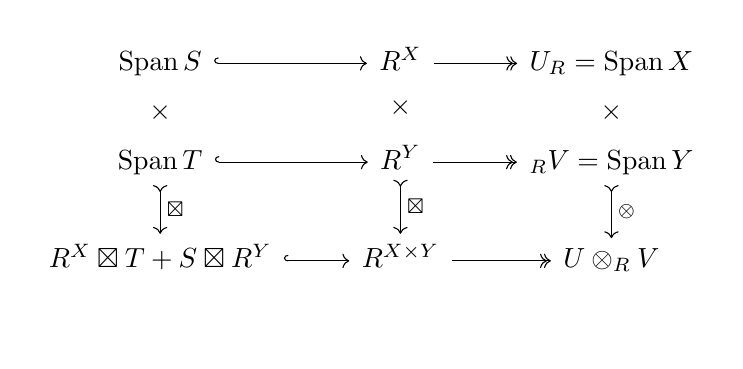
\begin{tikzpicture}
        \node at (0,0) {\begin{tikzcd}
            \Span S \arrow[d,phantom,"\times"]\arrow[r, hook] 
                & R^X\arrow[d,phantom,"\times"] \arrow[r,two heads] 
                    & U_R=\Span X\arrow[d,phantom,"\times"]  \\
            \Span T \arrow[r, hook]\arrow[d,"\boxtimes",tail] 
                & R^Y\arrow[d,"\boxtimes",tail] \arrow[r,two heads] 
                    & {_R V}=\Span Y\arrow[d,"\otimes",tail] \\            
            R^X\boxtimes T+S\boxtimes R^Y \arrow[r, hook] 
                 & R^{X\times Y} \arrow[r,two heads] 
                     & U\otimes_R V   \\
        \end{tikzcd}};
    \end{tikzpicture}
\end{frame}

\begin{frame}{Example}
    \[(\mathbb{Z}/2\mathbb{Z}\oplus \mathbb{Z}/6\mathbb{Z}\oplus \mathbb{Z})\otimes (\mathbb{Z}/4\mathbb{Z}\oplus \mathbb{Z}/8\mathbb{Z})\]
    \textbf{Solution.}
    \begin{align*}
        \left.
            \begin{bmatrix}\mathbb{Z} & \mathbb{Z}\\ \mathbb{Z} & \mathbb{Z} \\ \mathbb{Z} & \mathbb{Z} \end{bmatrix}
            \middle/
        \left(
            \begin{bmatrix} \mathbb{Z} \\ \mathbb{Z}\\ \mathbb{Z}\end{bmatrix}
        \begin{bmatrix} 4\mathbb{Z} & 8\mathbb{Z}\end{bmatrix}
        +
        \begin{bmatrix} 2\mathbb{Z} \\ 6\mathbb{Z}\\ 0\mathbb{Z}\end{bmatrix}
        \begin{bmatrix} \mathbb{Z} & \mathbb{Z}\end{bmatrix}\right)
        \right.\\
        =
        \left.
            \begin{bmatrix}\mathbb{Z} & \mathbb{Z}\\ \mathbb{Z} & \mathbb{Z} \\ \mathbb{Z} & \mathbb{Z} \end{bmatrix}
            \middle/
            \begin{bmatrix}4\mathbb{Z}+2\mathbb{Z} & 8\mathbb{Z}+2\mathbb{Z}\\ 4\mathbb{Z}+6\mathbb{Z} & 8\mathbb{Z}+6\mathbb{Z} \\ 4\mathbb{Z}+0\mathbb{Z} & 8\mathbb{Z}+0\mathbb{Z} \end{bmatrix}
        \right.\\
        =
        \begin{bmatrix}\mathbb{Z}/2\mathbb{Z} & \mathbb{Z}/2\mathbb{Z}\\ \mathbb{Z}/2\mathbb{Z} & \mathbb{Z}/2\mathbb{Z} \\ \mathbb{Z}/4\mathbb{Z} & \mathbb{Z}/8\mathbb{Z} \end{bmatrix}
    \end{align*}
\end{frame}

\begin{frame}
    $\mathbb{Z}/2\mathbb{Z}\otimes \mathbb{Q}$

    \begin{block}{Solution}
    $\mathbb{Q}=\left\langle \frac{1}{1!},\frac{1}{2!},\frac{1}{3!},\ldots\right\rangle =\langle e_1,e_2,\ldots \mid e_n=(n+1)e_{n+1}\rangle$
    \begin{align*}
        \left.
        \mathbb{Z}^{[1]\times \mathbb{N}}
        \middle/
        \left(2\mathbb{Z}\boxtimes \mathbb{Z}^{\mathbb{N}}
        +\mathbb{Z}\boxtimes \begin{bmatrix} 1 & -2 & & \\  & 1 & -3 & \\  & & \ddots & \ddots \end{bmatrix} 
        \right)
        \right.\\
        \only<6>{
            \left.
            \mathbb{Z}^{1\times \mathbb{N}}\middle/\mathbb{Z}\boxtimes \begin{bmatrix} 1 & -2 & & \\  & 1 & -3 & \\  & & \ddots & \ddots \end{bmatrix}
            \cong \mathbb{Q}
            \right.
        }
    \end{align*}
    \only<1-5>{
    \begin{align*}
        \begin{bmatrix} 1 & -2 & & \\  & 1 & -3 & \\  & & \ddots & \ddots \\ 2 & 0 \\ & 2 & 0 \\ & & \ddots & \ddots \end{bmatrix}
        \only<2>{\sim\begin{bmatrix} 1 & -2 & & \\  & 1 & -3 & \\  & & \ddots & \ddots \\ 0 & 4 \\ & 2 & 0 \\ & & \ddots & \ddots \end{bmatrix}}
        \only<3>{\sim\begin{bmatrix} 1 & -2 & & \\  & 1 & -3 & \\  & & \ddots & \ddots \\ 0 & 0 \\ & 2 & 0 \\ & & \ddots & \ddots \end{bmatrix}}
        \only<4>{\sim\begin{bmatrix} 1 & -2 & & \\  & 1 & -3 & \\  & & \ddots & \ddots \\ 0 & 0 \\ & 0 & 6 \\ & & \ddots & \ddots \end{bmatrix}}
        \only<5>{\sim\begin{bmatrix} 1 & -2 & & \\  & 1 & -3 & \\  & & \ddots & \ddots \\ 0 & 0 \\ & 0 &  0\\ & & \ddots & \ddots \end{bmatrix}}
    \end{align*}
    }

    \end{block}
    
\end{frame}

\subsection{Theory}

\begin{frame}{Theory}
    \only<1>{
    Tensor products are distributive
    \begin{align*}
        (u+\tilde{u})\otimes v & = u\otimes v+\tilde{u}\otimes v 
        \\
        u\otimes (v+\tilde{v}) & = u\otimes v+u\otimes \tilde{v}\\ 
        (U\oplus \tilde{U})\otimes_R V & = U\otimes_R V\oplus\tilde{U}\otimes_R V 
        \\
        U\otimes_R (V\oplus\tilde{V}) & = U\otimes_R V\oplus U\otimes \tilde{V}
    \end{align*}    
    }
    \only<2>{
        Tensor products have a 1.
    \begin{align*}
        U\otimes_R R & \cong U & R\otimes_R V \cong V
    \end{align*}
    }
    \only<3>{
    Sometimes it is said tensor products are associative and commutative, 
    \emph{that is nonsense}
    \begin{align*}
        \mathbb{R}^\otimes 
    \end{align*}
    
    But in special cases, e.g.\ if $R$ is \emph{commutative}
    \begin{align*}
        U\otimes_R (V\otimes_R W) \cong (U\otimes_R V)\otimes_R W\\
        U\otimes_R V & \cong V\otimes_R U.
    \end{align*}

    But be warned $U_1\otimes \cdots\otimes U_n$ is generally not defined!
    }
\end{frame}

\begin{frame}{Universal Mapping Property}
    Further fact $ur\boxtimes v=(ur)v^{\dagger}=u(rv)^{\dagger}=u\boxtimes rv$;\\
    so $ur\otimes v=u\otimes r v$.
    
    \begin{block}{Theorem}
        If $*:U\times V\bmto W$ is distributive and $\forall r\in R$, $ur*v=u*rv$ then $\exists ! \hat{*}:U\otimes_R V\to W$ where 
        \[
            u*v = \hat{*}(u\otimes v).
        \]
        In particular $U\otimes_R V$ does not depend on choice of presentations.
    \end{block}

    
\end{frame}

\begin{frame}{Whitney Tensor Product}

    Every module has its ``regular'' presentation
    \[ U_R=\Pres_R\langle e_u, u\in U \mid e_{u+\tilde{u}}=e_u+e_{\tilde{u}}, e_{ur}=e_u r\rangle
        \]
    \[ {_R V}=\Pres_R\langle e_v, v\in V\mid e_{v+\tilde{v}}=e_v+e_{\tilde{v}}, e_{rv}=re_v\rangle
        \]

    With these presentations we recover Whitney's definition (i.e. your textbook definition)
    \begin{align*}
        U\otimes_R V & = 
        \left.
        R^{U\times V}\middle/
        \left\langle \begin{array}{c}
        e_{u+\tilde{u}}\otimes e_v=e_u\otimes e_v+e_{\tilde{u}}\otimes e_v,\\
        e_u\otimes e_{v+\tilde{v}}=e_u\otimes e_v+e_u\otimes e_{\tilde{v}},\\
        e_{ur}\otimes e_v=e_u\otimes e_{rv}
        \end{array}\right\rangle
        \right.
    \end{align*}
    So established methods are a special case.
\end{frame}

\begin{frame}
    Similar ideas picking up on matrix-vector product $R^{m\times n}\times R^n\bmto R^m$ 
    give rise to 
    \[U\oslash V\times V\bmto U\] 

    Which behave like fractions, e.g.\ 
    \[ A\oslash K\cong A\qquad A\to K\oslash (K\oslash A)\]

    \[A\oslash (B\otimes C)=A\oslash B\oslash C\] 
    I.e.
    \[\hom(C\otimes B,A) \cong \hom(C,\hom(B,A))\]
\end{frame}

\section{Solving for Coordinates}

\begin{frame}
    
    \begin{block}{Applications}
        We \emph{have} a tensor.  Why would we want a tensor product?
    \end{block}

\end{frame}

\begin{frame}[fragile]
    What if $R=R_1\oplus R_2$?

    \centering
    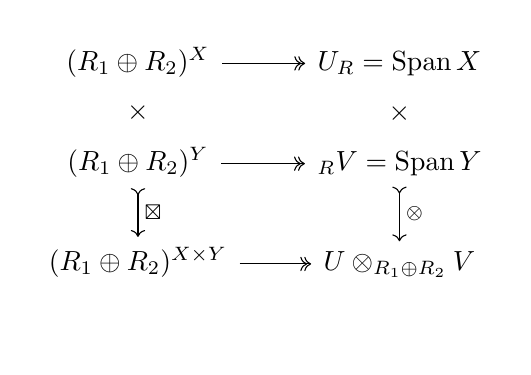
\begin{tikzpicture}
        \node at (0,0) {\begin{tikzcd}
            (R_1\oplus R_2)^X\arrow[d,phantom,"\times"] \arrow[r,two heads] 
                    & U_R=\Span X\arrow[d,phantom,"\times"]  \\
            (R_1\oplus R_2)^Y\arrow[d,"\boxtimes",tail] \arrow[r,two heads] 
                    & {_R V}=\Span Y\arrow[d,"\otimes",tail] \\            
            (R_1\oplus R_2)^{X\times Y} \arrow[r,two heads] 
                     & U\otimes_{R_1\oplus R_2} V   \\
        \end{tikzcd}};
    \end{tikzpicture}
\end{frame}

\begin{frame}[fragile]
    What if $R=R_1\oplus R_2$?

    \centering
    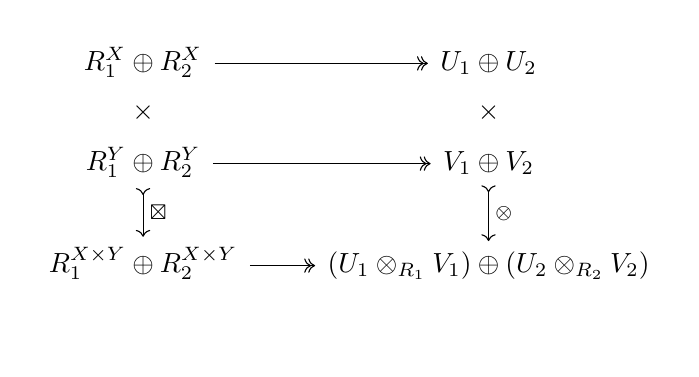
\begin{tikzpicture}
        \node at (0,0) {\begin{tikzcd}
            R_1^X\oplus R_2^X\arrow[d,phantom,"\times"] \arrow[r,two heads] 
                    & U_1\oplus U_2\arrow[d,phantom,"\times"]  \\
            R_1^Y\oplus R_2^Y\arrow[d,"\boxtimes",tail] \arrow[r,two heads] 
                    & V_1\oplus V_2\arrow[d,"\otimes",tail] \\            
            R_1^{X\times Y}\oplus R_2^{X\times Y} \arrow[r,two heads] 
                     & (U_1\otimes_{R_1} V_1)\oplus (U_2\otimes_{R_2} V_2)   \\
        \end{tikzcd}};
    \end{tikzpicture}
    
    That's one of these: 
    \pgfmathsetmacro{\xx}{0.5}
    \begin{tikzpicture}
			\pic at (\xx,-\xx,0) {shadedcube={\xx/\xx/\xx/gray/}};
			\pic at (0,0,\xx) {shadedcube={\xx/\xx/\xx/gray/}};
			\pic at (0,\xx,0) {opencube={2*\xx/-2*\xx/2*\xx}};
		\end{tikzpicture}
    ...for which people are hunting!
\end{frame}


\begin{frame}[fragile]
    Solve for \textbf{universal} $R$!

    \centering
    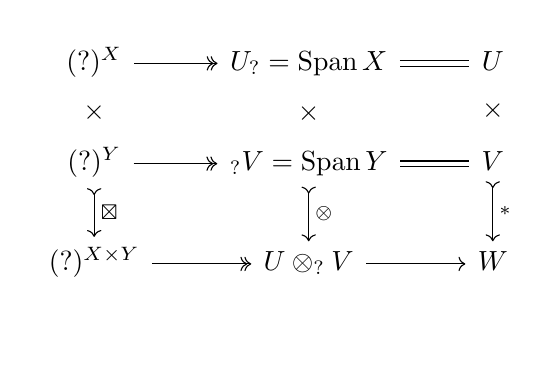
\begin{tikzpicture}
        \node at (0,0) {\begin{tikzcd}
            (?)^X\arrow[d,phantom,"\times"] \arrow[r,two heads] 
                    & U_?=\Span X\arrow[d,phantom,"\times"] \arrow[r,equal] 
                        & U\arrow[d,phantom,"\times"] \\
            (?)^Y\arrow[d,"\boxtimes",tail] \arrow[r,two heads] 
                    & {_? V}=\Span Y\arrow[d,"\otimes",tail] \arrow[r,equal]
                    & V\arrow[d,"*",tail]\\            
            (?)^{X\times Y} \arrow[r,two heads] 
                     & U\otimes_{?} V \arrow[r]
                        &  W\\
        \end{tikzcd}};
    \end{tikzpicture}

    Solution is the \textbf{Centroid}
    \[
        C(*)=\{(X,Y,Z)\mid Xu*v=Z(u*v)=u*(Yv)\}
    \]
\end{frame}

\begin{frame}{Cluster Algorithm (W. 2008)}
    $C(*)=\{(X,Y,Z)\mid  Xu*v=Z(u*v)=u*(Yv)\}$

    Random $\alpha\in C(*)$, \\
    if $\min_{\alpha}(x)=a(x) b(x)$ with $\deg a(x),\deg b(x)>0$ and 
    \[1=\mathrm{GCD}(a(x),b(x))=s(x)a(x)+t(x)b(x)\]

    Then $e = s(\alpha )a(\alpha)$; $f=t(\alpha)b(\alpha)$\\
    Return $U=eU\oplus fU$, $V=eV\oplus fV$, $W=eW\oplus fW$.\\
    
    Else try another $\alpha$. 

    \bigskip

    \textbf{Theorem W.} The resulting clusters are unique.

    %With constant number of trials you have decomposed or proven indecomposability.
\end{frame}


\section{Adjoints}

\begin{frame}
    \frametitle{Universal Property}

    \begin{block}{Theorem Brooksbank-Wilson.}
    The \textbf{adjoint algebra} is the largest set of operators 
    over which we can for tensor product.
    \end{block}
\end{frame}

\begin{frame}{Proof of Universality of Adjoints}
    \begin{proof}
        Suppose $\Omega\to \End(U)\times \End(V)^{op}$
    \end{proof}
\end{frame}

\end{document}